\documentclass[a4paper,12pt]{article}
\usepackage[margin=18mm]{geometry}
\usepackage{tikz}
\usepackage{amsmath}
\newcommand{\pFourCell}[1]{\makebox[2.7em][c]{\ensuremath{#1}}}
\pagestyle{empty}
\begin{document}
\section*{Spaltentreue LaTeX-Ausgabe}
\noindent Gleichung: \texttt{sin(x)/(2a)=5} \hfill Zielvariable: \texttt{x}

\vspace{8mm}
\begin{center}
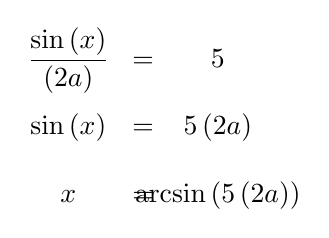
\begin{tikzpicture}[x=2.7em,y=-1em]
\node[anchor=base, inner sep=0pt] at (2,1) {$\displaystyle\frac{\pFourCell{\sin\left(x\right)}}{\pFourCell{\left(2 a\right)}}$};
\node[anchor=base, inner sep=0pt] at (3,1) {$=$};
\node[anchor=base, inner sep=0pt] at (4,1) {$5$};
\node[anchor=base, inner sep=0pt] at (2,3.45) {$\sin\left(x\right)$};
\node[anchor=base, inner sep=0pt] at (3,3.45) {$=$};
\node[anchor=base, inner sep=0pt] at (4,3.45) {$5\left(2 a\right)$};
\node[anchor=base, inner sep=0pt] at (2,5.9) {$x$};
\node[anchor=base, inner sep=0pt] at (3,5.9) {$=$};
\node[anchor=base, inner sep=0pt] at (4,5.9) {$\arcsin\left(5\left(2 a\right)\right)$};
\end{tikzpicture}
\end{center}

\newpage
\section*{Spaltentreue LaTeX-Ausgabe mit Raster}
\vspace{6mm}
\begin{center}
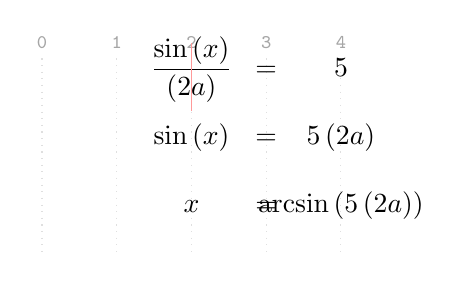
\begin{tikzpicture}[x=2.7em,y=-1em]
\draw[gray!25, dotted] (0,0.35) -- (0,7.45);
\node[font={\ttfamily\scriptsize}, text=gray!70, anchor=base] at (0,0) {0};
\draw[gray!25, dotted] (1,0.35) -- (1,7.45);
\node[font={\ttfamily\scriptsize}, text=gray!70, anchor=base] at (1,0) {1};
\draw[gray!25, dotted] (2,0.35) -- (2,7.45);
\node[font={\ttfamily\scriptsize}, text=gray!70, anchor=base] at (2,0) {2};
\draw[gray!25, dotted] (3,0.35) -- (3,7.45);
\node[font={\ttfamily\scriptsize}, text=gray!70, anchor=base] at (3,0) {3};
\draw[gray!25, dotted] (4,0.35) -- (4,7.45);
\node[font={\ttfamily\scriptsize}, text=gray!70, anchor=base] at (4,0) {4};
\node[anchor=base, inner sep=0pt] at (2,1) {$\displaystyle\frac{\pFourCell{\sin\left(x\right)}}{\pFourCell{\left(2 a\right)}}$};
\draw[red!40, line width=0.35pt] (2,-0.19999999999999996) -- (2,2.25);
\node[anchor=base, inner sep=0pt] at (3,1) {$=$};
\node[anchor=base, inner sep=0pt] at (4,1) {$5$};
\node[anchor=base, inner sep=0pt] at (2,3.45) {$\sin\left(x\right)$};
\node[anchor=base, inner sep=0pt] at (3,3.45) {$=$};
\node[anchor=base, inner sep=0pt] at (4,3.45) {$5\left(2 a\right)$};
\node[anchor=base, inner sep=0pt] at (2,5.9) {$x$};
\node[anchor=base, inner sep=0pt] at (3,5.9) {$=$};
\node[anchor=base, inner sep=0pt] at (4,5.9) {$\arcsin\left(5\left(2 a\right)\right)$};
\end{tikzpicture}
\end{center}
\end{document}
